\chapter{背景介绍}
  \section{中文拼音简介\label{sec:intro}}

  目前在中国大陆,一般的学前教育或者小学教育都是选汉语拼音作为中文教育的起点。汉语拼音,或又称拼音,是一种以拉丁字母作汉字标音的方案。\supercite{wjm}汉语拼音使用拉丁字母和标注在字母之上的一些附加符号来表示汉语发音。参考现代音韵学中对汉语音节结构的划分,可以将构成汉语拼音的成分分为声母、韵母和声调三部分。现代拼音输入法主要考虑声母和韵母两部分作为检索汉字的输入。

  按照汉语拼音方案《声母表》中的规定,声母由汉语中每一个音节的起始辅音构成。在中国诸多方言中,对辅音有不同程度的混合和模糊。如西南官话中的四川方言,对卷舌音和齿龈音不加区分,部分边音与鼻音不加区分;闽南语的泉漳片方言对唇齿音和软颚音音不加区分等等。\supercite{jdp}相对的,韵母主要由汉语中每一个音节的元音构成。按照韵母结构,又可将韵母分为单韵母、复韵母和鼻韵母三类。

  在汉语拼音系统中,还有语流音变现象,包括变调、轻声、儿化、音变等等。但这些现象在现代汉语输入法中均没有得到使用,在此略过不谈。

  \section{现有输入法简介\label{sec:current_input}}

  中文输入法是一种重要的人机交互方式。有别于拉丁字母数量少,编码简单,中文字符必须经过合理的编码和科学的设计才能使输入方便快捷。现代主流的输入法种类繁多,根据输入方式分类,主要可以分为键盘输入、语音输入和手写输入等。

  语音输入是指机器通过识别用户输入的声音信号,输入用户想要表达的汉字的过程。其中涉及到机器学习,音频分析等等技术。近年来,中文语音输入得到了极大地发展。如,Lee等人\supercite{lee5system, lee1997voice, lee1993mandarin}用语音建模,语义建模和声音识别建模的方法,对中文语音输入做出了大量贡献。然而,目前语音输入依然存在一些主要问题亟需解决:如各方言语音的适配不足导致的识别率不高\supercite{chen2000tone};汉字同音字较多,需要上下文语义判断具体汉字,或需手动选择汉字;语音处理和语义判断逻辑复杂,需要的语料库庞大等等。这些问题降低了输入速度和精度,也增加了用户的负担。

  手写输入相对于语音输入,比较成熟,识别率较之语音输入也较高。然而,手写输入的一大缺点是输入速度难以提升。日常生活中,我们想要提高书写汉字的速度最直接的方法就是笔画连写,而对目前的汉字识别技术,笔画连写会对识别率造成比较大的影响。\supercite{srihari2007offline}当然,长时间的手写输入对用户也是一种负担。

  键盘输入是最常用的中文输入方式。其主要思路是将中文汉字的特征编码加工,从而映射到键盘的不同按键上。当用户敲击对应按键时,输入相应特征的文字。键盘输入主要分为拼音输入法、形码输入法(五笔、郑码)和音形码输入法(二笔、自然码)。\supercite{wgy, dsl}其中汉语拼音输入法在键盘输入法中占有着统治地位,97\%的用户选择拼音输入法作为自己的主要输入法。\supercite{chen}汉语拼音输入法也是本文讨论的重点。

  \subsection{现有拼音输入法的局限性\label{sec:limit}}

  \begin{enumerate}

  \item
  键盘布局非最优:按照键盘布局分类,主流拼音输入法可以分为九键键盘和QWERTY键盘两种。而九键键盘的设计源自于手机键盘,与QWERTY键盘一样,最初都是为输入拉丁字母而设计。笔者写了一个简单地程序\footnote{\url{http://hacker-yhj.github.io/projects/keyboardStroke/index.html}}统计了英文资料与中文资料在QWERTY键盘上使用的热度(考虑中文资料使用拼音输入)。结果如图\ref{fig:stats_en}和图\ref{fig:stats_cn}所示。可以看出中英文输入对键盘的使用情况差异比较大,中文的统计数据的方差值较大,分布更为分散。这意味着使用QWERTY键盘作为中文输入,手指所需做的操作更多,给用户的负担更大。

  \begin{figure}[h]
  \noindent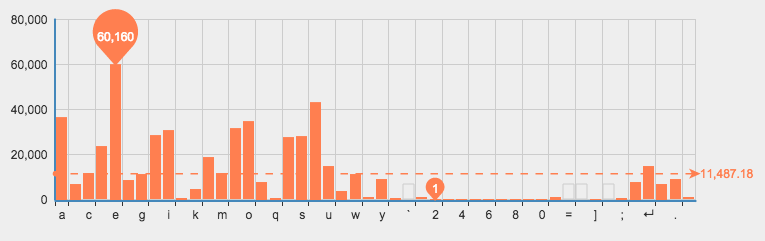
\includegraphics[width=150mm]{img/stats_en}
  \caption{英文资料键位统计图}
  \label{fig:stats_en}
  \end{figure}

  \begin{figure}[h]
  \noindent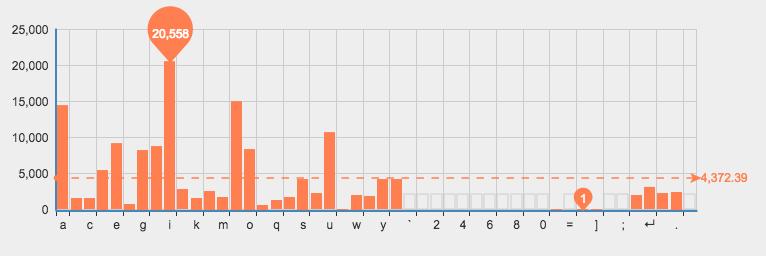
\includegraphics[width=150mm]{img/stats_cn}
  \caption{中文资料键位统计图}
  \label{fig:stats_cn}
  \end{figure}

  \item
  回忆式操作门槛高:拼音输入法要求用户使用之前熟练掌握汉语拼音,不仅如此,还要求用户熟悉每一个汉字的对应拼音组合。结合对键盘布局的考虑,还需要用户熟悉一套键盘设计,了解每一个键的位置。这无疑会增加用户的学习和记忆的负担,对于汉语的初学者来说更是“望洋兴叹”。

  \item
  输入错误修改频繁:用户在使用现有输入法时,往往需要键入声母和韵母之后,浏览过候选汉字,才能意识到自己的输入有误。此时修改输入往往需要连续使用退格键,返回出错位置。这种重复并低效的操作大大影响了用户的输入速度和连续性。

  \item
  声母韵母易混淆:目前所有的拼音输入法均要求用户使用先声母后韵母的输入方式。对某些方言地区的用户来说,分辨声母是很困难的,结合对输入错误修改频繁的讨论,一旦发现输入有误,用户必须删除韵母部分才能修改声母部分。
  \end{enumerate}

  \subsection{现代拼音输入法的新特性\label{sec:new_feature}}

  很多现代拼音输入法做了很多辅助性的工作,意在为用户提供更好地输入体验。

  \begin{enumerate}

  \item
  输入消歧:事实上,拼音作为汉字输入法编码时,重码率非常的高。在GB2312字符集单字重码率上,像五笔、二笔和郑码的重码率都低于5\%,而汉语拼音的编码重码率高达94\%,即使词组重码率上,形码或音形码重码率仍然要比拼音编码重码率低得多。一些研究从结合上下文语义、机器学习等方向对该问题做出了改善。\supercite{wen2008ambiguity, liu2002approach}

  \item
  模糊音:对于不通话不标准的方言地区用户,对常见的易混淆的声母韵母进行了分类。当用户选择开启某一类模糊音选项时,输入法对该选项中的所有易混淆项不加区分。

  \item
  整句输入:随着使用拼音输入法的用户对拼音输入的熟练度逐渐提高,对多字和整句输入的需求明显变高。主流输入法都支持连续输入声母韵母对来输入长句子,不仅增加了输入速度,也能通过上下文语义来消除歧义。

  \item
  生僻字输入:对于不知道读音的生僻字,某一些输入法支持将其从字形上拆解成两个汉字进行输入,只需在输入前加入“u”这个不能作为普通汉字开头的字母即可。如“垚”,输入法下键入“utututu”就可以检索到这个字。
  \end{enumerate}
